\chapter{Results}
\chlab{results}

For the user studies, we invited a total of 16 chemistry researchers. They come from various institutes, but the majority works at VU University Amsterdam or the University of Queensland, Australia. Half of the invited received the instructions for the \IDa-first version of the experiment, the other half was instructed to use the \IDb\ version first.

Out of all the invited people, 10 fully completed their tasks and submitted the results they obtained. 6 of them used the \IDa\ version first, the other 4 started with the \IDb\ version. Unfortunately, it is impossible to tell how many people started the experiment, but did not finish it, as the log files were only uploaded to the server after completing a version's questionnaire. However, we observed that there were no people who only completed one of the two versions.

A lot of different types of data have been gathered. Graphical representations of most observations from the user action log can be found in \appref{graphs}. In that same chapter, one can find the outcomes of the \verb|SUS| and \verb|UMUX| questions that were asked in the questionnaire as well. \Appref{comments} contains all answers to the open questions, including general comments about the system, the preferred version and suggestions for improvement.

In this chapter, we present the important and most interesting results obtained from the user studies. Each result will shortly be discussed, and further analysed in \chref{discussion}. Some additional results are provided in \appref{results_extra}.



\section{Action log results}
From the logging system that was built into \oframp{} for the user studies, a wide range of information can be gathered, spanning from the load time and the number of clicks on atom 5 to the selected conflict solutions and resulting parameterisation. In this section, we present the most interesting results that can be retrieved from the action log.


\subsection{Time required}
\seclab{res_time}
First of all, it is interesting to see in which version users spent the most time to fully parameterise the molecules. \Figref{graph_time_1} shows the total time that was required for both the first and second set of molecules, in both the \IDa\ and \IDb\ version of \oframp. Note that here, and in the subsequent graphs, the group that did the \IDa\ version first is the same group of people that did the \IDb\ version second, and vice versa for the other group.

\begin{figure}[h!]
\center
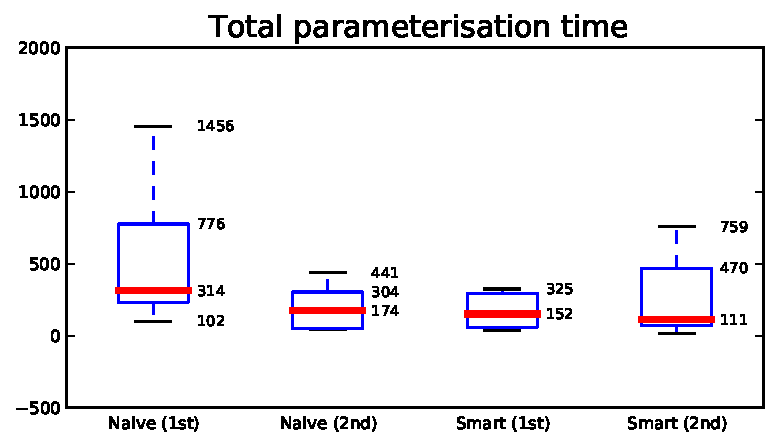
\includegraphics[width=.6\textwidth]{img/graphs/1a_02.pdf}
\caption{Total time for the \nth{1} and \nth{2} set of molecules for both versions.}
\figlab{graph_time_1}
\end{figure}

What can be seen in \figref{graph_time_1} is that, for both the first and second set of molecules, users needed more time to complete the parameterisation using the \IDa\ version. Users who started with the \IDa\ version used the most time overall, with a median total time of around 300 seconds. Those same users spent the least time on the \IDb\ version, where the median time value is around 100 seconds. At around 150 and 180 seconds, one can find the median times required by the users who did the \IDb\ version first and the \IDa\ version second respectively.

The total time used to parameterise the first and second sets of molecules can be used to determine which version of \oframp{} is the most time-consuming. However, as both sets of molecules have slightly varying molecule sizes, it may be more interesting to look at the average time that was required per atom. This can be seen in \figref{graph_time_2}.

\begin{figure}[h!]
\center
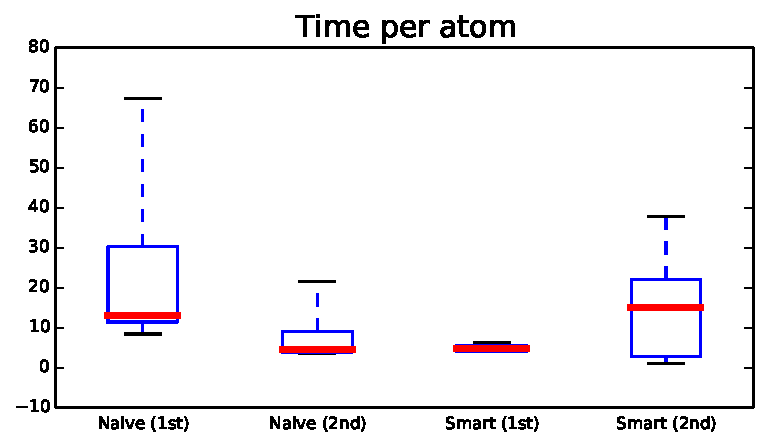
\includegraphics[width=.6\textwidth]{img/graphs/1a_03.pdf}
\caption{Average time per atom for the \nth{1} and \nth{2} set of molecules for both versions.}
\figlab{graph_time_2}
\end{figure}

What is interesting to see here, is the fact that, where in the total parameterisation time, the group that did the \IDb\ version second was done the fastest, its members have spent the most time on average per atom. When taking a closer look at \figref{graph_time_3, graph_time_4}, which show the average time per atom for all molecules separately, this difference appears to be caused completely by the excessive amount of time users spent on parameterising molecule 13913 in the \IDb\ version. This is the first molecule users got to parameterise after they completed the \IDa\ variant.

\begin{figure}[h!]
\centering
\begin{subfigure}[t]{0.48\textwidth}
\centering
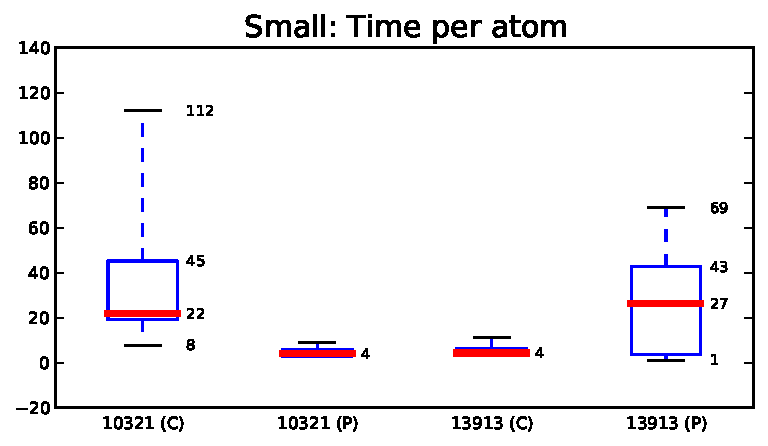
\includegraphics[width=\textwidth]{img/graphs/1c_03.pdf}
\caption{Smaller molecules.}
\figlab{graph_time_3}
\end{subfigure}%
~
\begin{subfigure}[t]{0.48\textwidth}
\centering
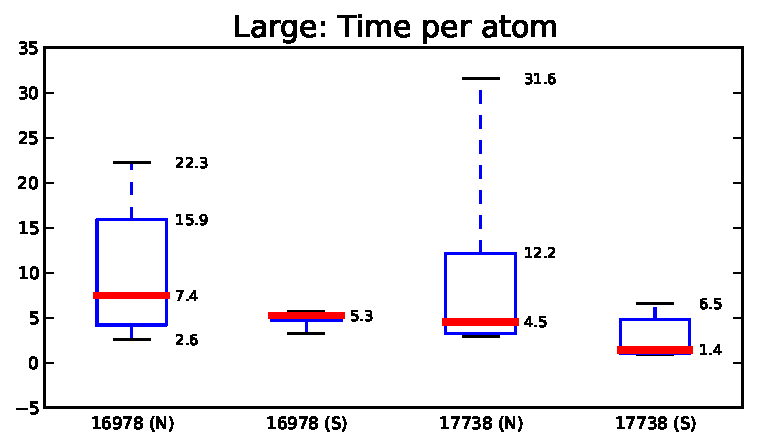
\includegraphics[width=\textwidth]{img/graphs/1d_03.pdf}
\caption{Larger molecules.}
\figlab{graph_time_4}
\end{subfigure}
\caption{Average time per atom for all molecules for both versions.}
\figlab{graph_time_34}
\end{figure}

It is hard to say what exactly is causing this difference. It is possible that, after using the \IDa\ version, it is hard to get used to the \IDb\ version, which is way more restrictive as to what a user can do. This difference is not present when switching from the \IDb\ to the \IDa\ version, which can either mean that this switch is easier to make, or that there must be a different cause of the large time difference.

Another possible explanation for the large increase in time required for parameterising molecule 13913 is that good matching fragments may not occur in the used repository, enforcing the user to browse through many of them before finding an acceptable one. This is better facilitated by the \IDa\ version of the tool, and can potentially have the extreme effects that are observed here.


\subsection{Parameterisation rating}
\seclab{res_rating}

Not only the time required by the parameterisation tool can be used to assess the two interaction designs, the quality of the result is also of great importance. As discussed in \secref{ev_analysis}, there are two ways of calculating this quality rating. First, the total difference between the charge found by the user and the charge present in the ATB is shown in \figref{graph_rating_1}. As this difference can easily be observed and corrected by the user, it would be expected that it would be relatively close to 0. This, however, turns out not to be the case. Especially in the \IDb\ version of \oframp, the charge difference can get quite high, and is greater than the charge difference for the \IDa\ version in any case.

\begin{figure}[h!]
\center
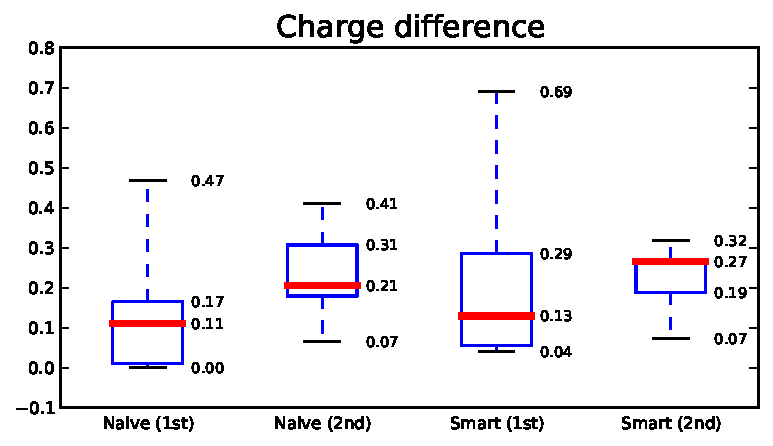
\includegraphics[width=.6\textwidth]{img/graphs/1a_00.pdf}
\caption{Total charge difference for the \nth{1} and \nth{2} set of molecules for both versions.}
\figlab{graph_rating_1}
\end{figure}

What is also interesting to note here is the fact that, for both the \IDa\ and the \IDb\ version of \oframp, the total charge difference is higher for the second set of molecules. This may indicate that these molecules are harder to parameterise, or that there are no good matching fragments available for those molecules. However, it may also indicate that users were starting to lose their concentration, or were confused due to the switch from one version to another.

Whereas the difference in the total molecule charge can mainly be used to assess user performance, the correctness of the parameterisation can better be measured using the per-atom charge differences. \Figref{graph_rating_2} shows these differences for the first and second set of molecules, both for the \IDa\ and \IDb\ version of \oframp. As can be seen in that graph, charge differences are, again, smaller for the \IDa\ version than they are for the \IDb\ version.

\begin{figure}[h!]
\center
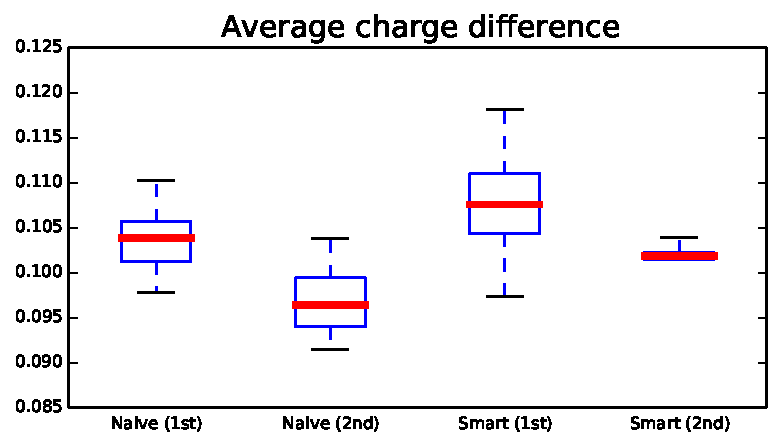
\includegraphics[width=.6\textwidth]{img/graphs/1a_01.pdf}
\caption{Average charge difference for the \nth{1} and \nth{2} set of molecules for both versions.}
\figlab{graph_rating_2}
\end{figure}

In contrast to the total charge differences though, the average charge differences for the second set of molecules are smaller than those for the first set. This suggests the opposite of what was concluded from \figref{graph_rating_1}: the second set of molecules may be easier to parameterise, or there may be better matching fragments available. This suggestion is more probable, as, for the total charge difference, a negative offset between two atom charges can be compensated by a positive offset in two others. This is not the case for the per-atom difference.

As can be seen in \figref{graph_rating_34}, the \IDa\ version of \oframp{} scores better for all individual molecules. What can also be seen there is the fact that, even on average, the charge differences are bigger for the larger molecules than for the smaller ones. Unfortunately, there is no obvious explanation for this. Probably, larger fragments are used for the larger molecules. When one of those fragments is bad, it quickly adds up to the atom charge difference. On the other hand, it is also possible that users felt more comfortable selecting small fragments, which are generally worse matches than the large ones, due to less atoms matching between the two molecules.

\begin{figure}[h!]
\centering
\begin{subfigure}[t]{0.48\textwidth}
\centering
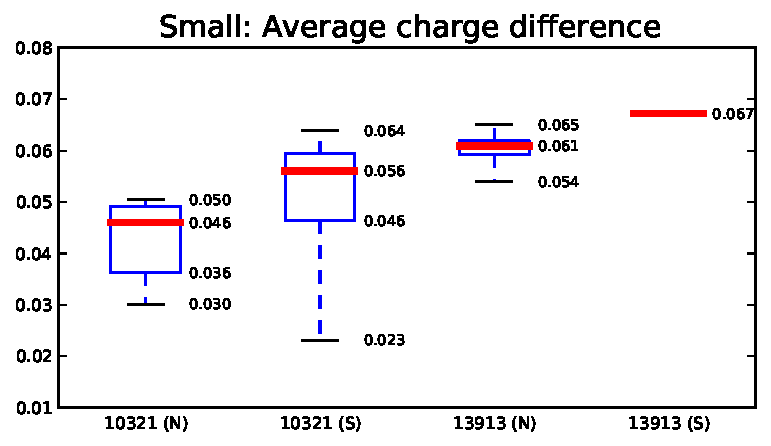
\includegraphics[width=\textwidth]{img/graphs/1c_01.pdf}
\caption{Smaller molecules.}
\figlab{graph_rating_3}
\end{subfigure}%
~
\begin{subfigure}[t]{0.48\textwidth}
\centering
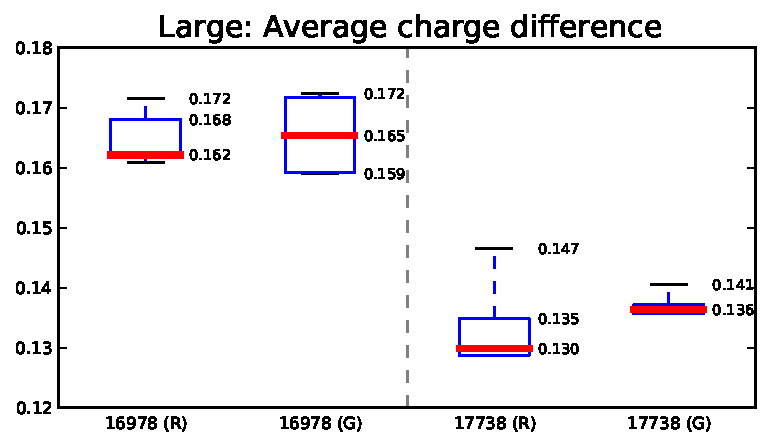
\includegraphics[width=\textwidth]{img/graphs/1d_01.pdf}
\caption{Larger molecules.}
\figlab{graph_rating_4}
\end{subfigure}
\caption{Average charge difference per atom for all molecules for both versions.}
\figlab{graph_rating_34}
\end{figure}


\subsection{Other results}
\seclab{res_other}

Besides the time required to complete the parameterisation and its rating, some other interesting things were observed in the user studies. First of all, there appears to be a great correlation between the version of \oframp{} that is used and the amount of actions a user needs to undo, as we can see in \figref{graph_undo}. Where, in the \IDa\ version, users practically do not undo any action, there are extreme cases where a user undid over a hundred actions in the \IDb\ version. This difference can be explained by the fact that users of the \IDb\ version have to undo accidentally rejected fragments, or may use a combination of reject and undo actions to compare various fragments.

\begin{figure}[h!]
\center
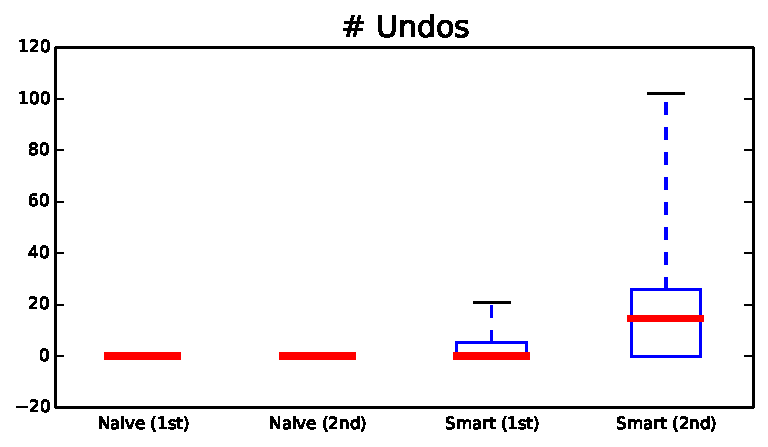
\includegraphics[width=.6\textwidth]{img/graphs/1a_10.pdf}
\caption{Number of undo actions for the \nth{1} and \nth{2} set of molecules for both versions.}
\figlab{graph_undo}
\end{figure}

As can be seen in \figref{graph_clicks}, a few more clicks are required to complete a parameterisation in the \IDb\ version of the tool, than in the \IDa\ version. Nevertheless, the medians are not too far apart, so it is not really possible to draw any conclusions from this. It is interesting to see, however, that even though the \IDb\ version of \oframp{} requires less user interaction, is does not require less, and possibly even more clicks to complete a parameterisation.

\begin{figure}[h!]
\center
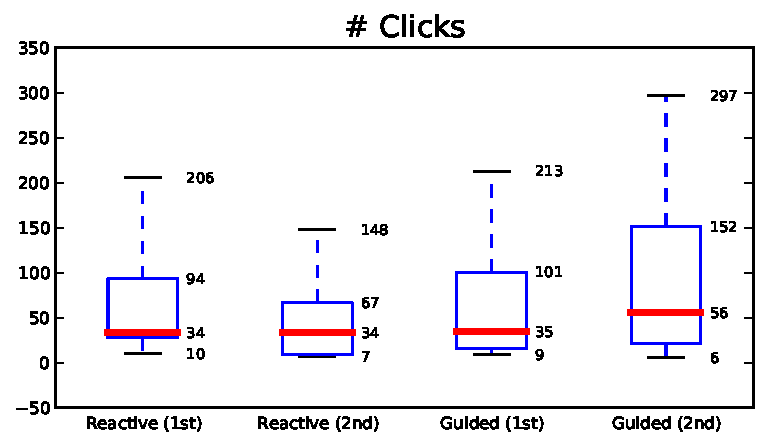
\includegraphics[width=.6\textwidth]{img/graphs/1a_04.pdf}
\caption{Total number of clicks for the \nth{1} and \nth{2} set of molecules for both versions.}
\figlab{graph_clicks}
\end{figure}

\Figref{graph_help} shows that not many users consulted the help pages during the parameterisation process, even though they were made aware of their existence. Furthermore, no users checked the help pages in their second version of the system. This can mean that either they did not know there were different versions of the help pages, or they did not need it any more. The fact that most users did not go to the help pages at all suggests that the tool is intuitive to use, and that taking the demo provides enough information to be able to use \oframp.

\begin{figure}[h!]
\center
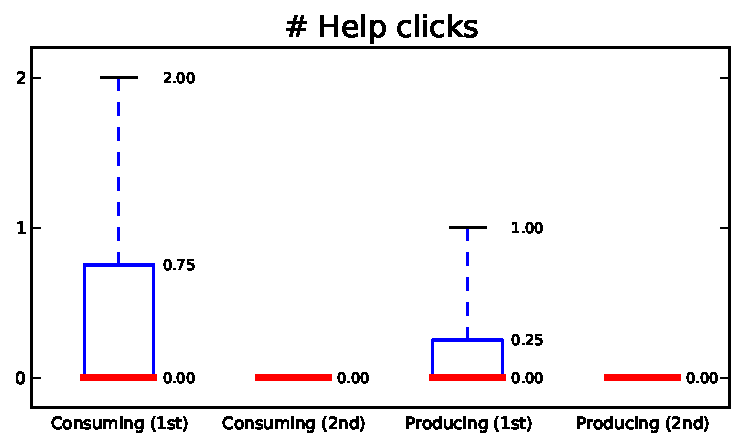
\includegraphics[width=.6\textwidth]{img/graphs/1b_01.pdf}
\caption{Total number of clicks on the help button for the \nth{1} and \nth{2} set of molecules for both versions.}
\figlab{graph_help}
\end{figure}

There are also a few things users did not do at all. They were not required or instructed to use every aspect of \oframp, but it was expected that they would at least try some of the more advanced features. First, none of the users used any of the available keyboard shortcuts. Although all actions for which a keyboard shortcut exists can also be completed using a single mouse click, it was expected that some users would find it beneficial to use keyboard shortcuts for some actions.

Furthermore, and more surprisingly, none of the users manually edited a single atom charge. Again, they were not specifically instructed to do so, but they were made aware of the possibility of doing this, and instructed to make the parameterisation as good as possible. Possibly, they just did not feel the need of it, or thought their parameterisation was perfect the way it was. However, as we will see later in \secref{res_comments}, some users commented they would like to see the possibility of manually editing atom charges added to the system, suggesting otherwise.



\section{Questionnaire outcomes}
\oframp\ can also be evaluated using the information gathered from the questionnaire users were asked to fill in. This includes the results of the combined \verb|SUS| / \verb|UMUX| questionnaire, their preference verdict on the two versions, and other comments about the system. We will discuss all of these in the next sections.


\subsection{\texttt{SUS} / \texttt{UMUX} results}
\seclab{res_sus}
The total \verb|SUS| score of the \IDa\ and \IDb\ versions of the system is shown in \figref{graph_sus_1}. As can be seen here, the \IDa\ version, with a median rating of $76$, scores better than the \IDb\ version, which has a median rating of only $61$. This means that the \IDa\ version scores above the average \verb|SUS| score of 68~\cite{sauro2011measuring}, where the \IDb\ version scores below that. In the adjective rating scale, the \IDa\ version is `good', but the \IDb\ version still scores `OK'~\cite{bangor2009determining}~(see also \secref{ev_analysis}).

\begin{figure}[h!]
\center
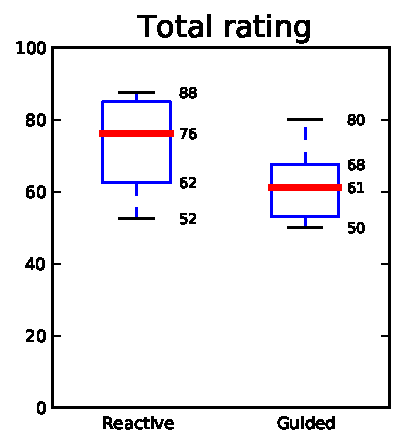
\includegraphics[width=.32\textwidth]{img/graphs/4a_10.pdf}
\caption{\texttt{SUS} score of the two versions.}
\figlab{graph_sus_1}
\end{figure}

\Figref{graph_sus_2} shows the ratings separately for the two different orders in which the users used the two versions of \oframp~(\verb|RF| for \IDa-first and \verb|GF| for \IDb-first). Here, the outcomes are slightly different. First of all, it appears that the group that did the \IDa\ version first was less positive in general. With a median grade of only 62, the \IDa\ version scores below average and is rated as just `OK'. Although it is still rated higher than the \IDb\ version, with outliers to very high ratings, the difference in the medians is very small and not really significant.

\begin{figure}[h!]
\center
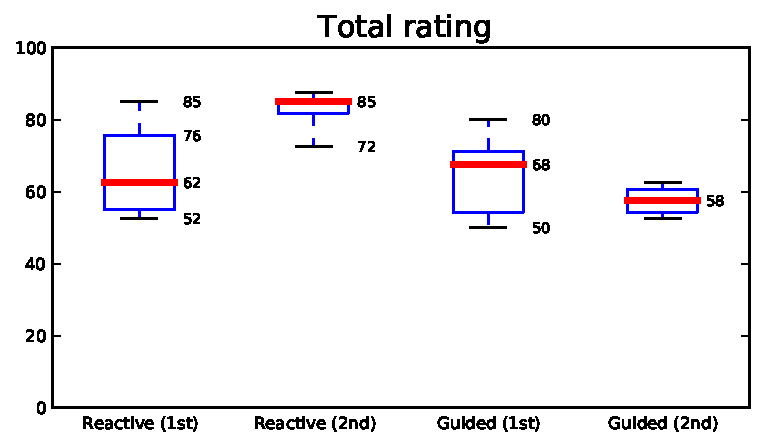
\includegraphics[width=.6\textwidth]{img/graphs/4b_10.pdf}
\caption{\texttt{SUS} score of the two groups for both versions.}
\figlab{graph_sus_2}
\end{figure}

For the other group of users, the opposite is true. They already awarded the \IDb\ version with the average grade of $68$, and later rewarded the \IDa\ version with a rating of $85$, which translates to `excellent' on the adjective scale. This large difference can possibly be explained by the users preferring the \IDa\ version over the \IDb\ one and therefore, consciously or unconsciously, giving it higher grades. The lower, but still `OK' grading of the \IDb\ version in the other group can then be explained by the users still liking that version, and therefore willing to grade it sufficiently.

The most extremely rated \verb|SUS| questions are shown in \figref{graph_sus_345}. \Figref{graph_sus_3} shows the lowest scoring point for both the \IDa\ and the \IDb\ versions of \oframp, being the answer to the first \verb|SUS| statement: ``I think that I would like to use this system frequently''. Whereas, for the \IDa\ version, most people are neutral, with some agreeing or even fully agreeing with the statement, the median answer in the \IDb\ version was a disagree. This is an important result, as users not liking to use a system frequently is, of course, a bad sign.

\begin{figure}[h!]
\centering
\begin{subfigure}[t]{0.32\textwidth}
\centering
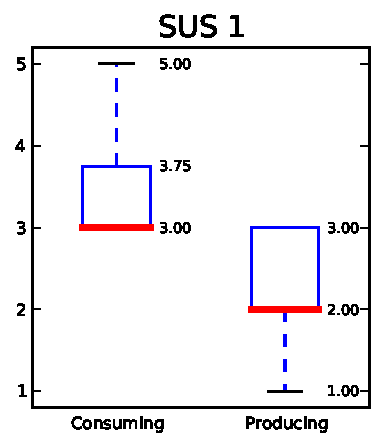
\includegraphics[width=\textwidth]{img/graphs/4a_00.pdf}
\caption{Rating of \texttt{SUS1}.}
\figlab{graph_sus_3}
\end{subfigure}%
~
\begin{subfigure}[t]{0.32\textwidth}
\centering
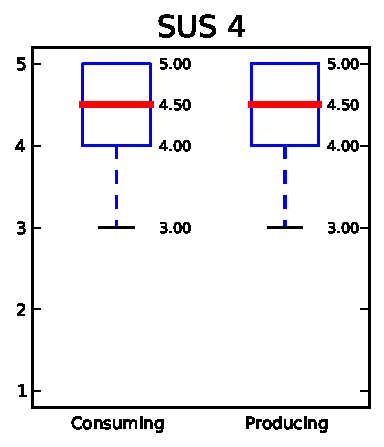
\includegraphics[width=\textwidth]{img/graphs/4a_03.pdf}
\caption{Rating of \texttt{SUS4}.}
\figlab{graph_sus_4}
\end{subfigure}%
~
\begin{subfigure}[t]{0.32\textwidth}
\centering
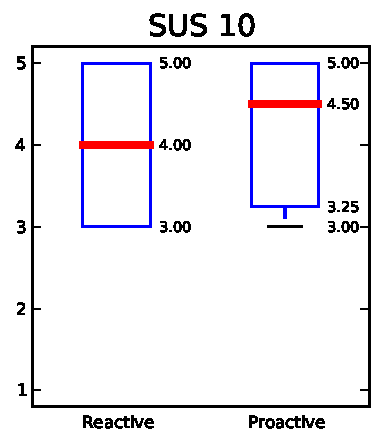
\includegraphics[width=\textwidth]{img/graphs/4a_09.pdf}
\caption{Rating of \texttt{SUS10}.}
\figlab{graph_sus_5}
\end{subfigure}
\caption{Selected ratings for the two versions of \oframp.}
\figlab{graph_sus_345}
\end{figure}

The fourth \verb|SUS| question was the highest rated for both the \IDa\ and \IDb\ versions of the system~(see \figref{graph_sus_4}), although the tenth question is rated equally high in the \IDb\ version. \verb|SUS4| states: ``I found the various functions in the system were well integrated''. As there is no difference in the rating of the two versions, no conclusions can be drawn for this, other than the fact that both interaction designs are well-integrated in general.

Finally, as mentioned before, the tenth \verb|SUS| question is one of the highest rated for the \IDb\ version. Furthermore, this is the only statement for which the \IDb\ version actually scores higher than the \IDa\ one. As the tenth statement is ``I think the system meets up with its requirements'', it is quite interesting that the \IDb\ version scores higher here. Probably, the test participants considered the required time to complete the parameterisation an important requirement. As seen before, the \IDb\ version requires the least time, which may explain the difference here.


\subsection{Preference}
\seclab{res_preference}
The general questionnaire users were asked to submit after they were completely done started off with the question which version of the system they preferred. All participants actually preferred the \IDa\ version, no matter whether they had to use that first or last. Most users commented that they felt they had more control over the parameterisation process in that version, which they thought they really needed. Furthermore, they preferred seeing a list of possible matches over the accept/reject system.

Additionally, some users commented that the \IDa\ version allowed for easier comparison of fragments, compared to having to make a combination of rejects and undos in the \IDb\ version. One user even commented this made the parameterisation process a lot quicker, though the timing results discussed before tell a different story. This means that the \IDa\ version \emph{feels} faster, and suggests that the parameterisation process using the \IDb\ version may be considered to be tedious.


\subsection{Comments}
\seclab{res_comments}
Following the \verb|SUS| and \verb|UMUX| questions, users were asked to answer a few open questions and had room for some comments. In the next sections, we will discuss these comments for both versions of \oframp{} and the suggestions they had for improving the tool. As we have not observe any significant difference between the comments of the people for the different orders in which they used the system, no distinction will be made between those comments.

\subsubsection{\IDA\ version}
For the \IDa\ version of the system, users were very positive about the user interaction. They noted that the interface and layout were very clear and nicely designed, and also gave a nice representation of molecules and fragments. The interface was found to be very responsive and easy to use and learn, thanks to the demo mode, the extensive help pages, and the fact that the system was intuitive to use in general. Finally, the right information was noted to come up exactly when needed.

Users were also enthusiastic about the chemical concepts behind \oframp. They liked the idea of fragment-based molecule parameterisation in general, and specifically the fact that this allows them to iteratively assign charges to a molecule. Furthermore, they found that there was a good variety of fragments available to complete the parameterisation. However, the ordering of these fragments could use some work, as the highest rated ones are in fact rarely the best available matches. It was also commented that using a shell around the atoms to find matching fragments may not be the best way to find good matches, as this will not detect all atomic properties.

There were some critical notes about the user interface as well. Some users found the `finished' popup confusing and annoying. A few users commented that it was hard to keep track of the total molecule charge, and that this should be visible at all times. Others had trouble finding out how to scroll the list of found fragments, presumably due to the alternatively styled scrollbars.

There were also some disagreements between different users. Where some really liked the colour coding of the atoms, and especially the indication of the conflicting fragments, others found the used colours confusing and suggested using different ones. It was also noted that it made no real sense for users to manually decide which (group of) atoms needed to be selected, while others highly valued this.

Finally, many users noted that they would like to be able to manually alter or insert charges for certain atoms. As was already suspected from the analysis of the action logs, users did not find the charge edit functionality in the selection details window. A user also commented that it should be possible to see what fragments have been used to parameterise an atom. This is available in the same place where the charges can be edited, and further confirms the idea that this has to be positioned in a more prominent spot, or indicated in a better way.

\subsubsection{\IDB\ version}
In their comments about the \IDb\ version of \oframp, users were, again, quite positive about the interface. They noted it to be clear and running smooth, and liked the visualisation of the molecule. Additionally, they found the tool extremely easy to learn, and mentioned it helped them to parameterise a molecule very quickly. It was mentioned again that fragment-based molecule parameterisation is a good concept to speed up molecule parameterisation. Finally, the ability to view the original molecule was found to be truly valuable.

Despite all the positive feedback, all users encountered one major problem: they were not able to easily compare different fragments. This either resulted in them having to go through some sort of reject/undo loop, or made them select a fragment before they were confident that it was the best available. Furthermore, they noted that taking the average of the conflicting atom charges is not always a good solution, and they needed to be able to decide how the conflict should be solved. Some users also commented that the automatic atom selection was too arbitrary, and needed to be more intelligent.

Most of the shortcomings of the \IDa\ version were also mentioned here. Again, many noted that they needed to have an easy way to keep track of the total molecule charge. Some found the `finished' popup obstructive, and it was mentioned once more that making matches based on a shell around the target atoms may not be the best approach.

\subsubsection{Suggestions for improvement}
\seclab{res_suggestions}
Many users had some ideas for further improving the value of \oframp. The following list contains the most mentioned and feasible ones, ordered on descending number of mentions.
\begin{enumerate}
\item Continuously show the total molecule charge:\\
Even though the molecule charge can be viewed in the selection details window, this window is not opened at all times. Additionally, the effect of selecting a proposed fragment on the total charge can be shown with it;
\item Ability to manually add/edit charges:\\
As discussed before, many users wanted to see this feature added, even though it is already present. Additionally though, they commented that they would like to be able to assign a charge to a group of atoms, and have this automatically distributed over the group;
\item Combine the auto-select system with the fragment list:\\
Some users noted they did not want to manually select atoms all the time, and liked the automatic selection system from the \IDb\ version. As this was lacking the overview of fragments, they wanted to combine it with the list of fragments from the \IDa\ version to make the ultimate parameterisation system;
\item Show the confidence score of fragments:\\
It was noted a few times that this would help in finding the best available fragment;
\item Indicate identical sections in the atom that is being parameterised:\\
In some molecules, sections of atoms occur multiple times. For these sections, the charges are generally equal. It would therefore be useful if these sections would be highlighted and will probably be useful to copy the charges automatically;
\item Remember the position of the popup:\\
As the popup location is reset every time, users have to move it to the side every time they want to compare an original molecule to the input molecule. Some therefore consider it better to remember the location the popup was dragged to once it is reopened;
\item Colour coding of atom types:\\
It has been noted to be common practice in chemistry applications to colour code atoms based on their type. Some users would like to see that in \oframp{} as well.
\end{enumerate}
